
\section{Simterpose: la médiation / Simterpose: les actions sur lesquelles faire de la médiation}
\label{section:simterpose}
Dans le cadre du projet Simterpose de virtualisation légère et de test
d'applications distribuées, c'est l'émulation par interception qui a été
choisi. En effet, le but final étant de pouvoir évaluer n'importe quelle
application distribuée sur n'importe quel type d'architecture, on pourrait se
retrouver à devoir émuler des machines plus puissantes que l'hôte, ce que
l'émulation par dégradation ne permet pas. Pour cela on va utiliser SIMGRID
comme simulateur et Simterpose comme émulateur. Simterpose qui est une API de
SIMGRID nous permettra donc d'utiliser le simulateur avec des applications
réelles tout en leur faisant croire qu'elles s'exécutent sur des machines
distinctes. Simterpose étant l'émulateur qui va nous permettre d'intercepter les
communications de l'application avec la machine sur laquelle elle s'exécute et
de faire de la médiation, nous allons étudier son fonctionnement et voir quels
outils présentés en section \ref{section:emulation} ont été choisis.

\subsection{Organisation générale}
%schéma tableau
%% \begin{figure}[H]
%%  \centering
%%  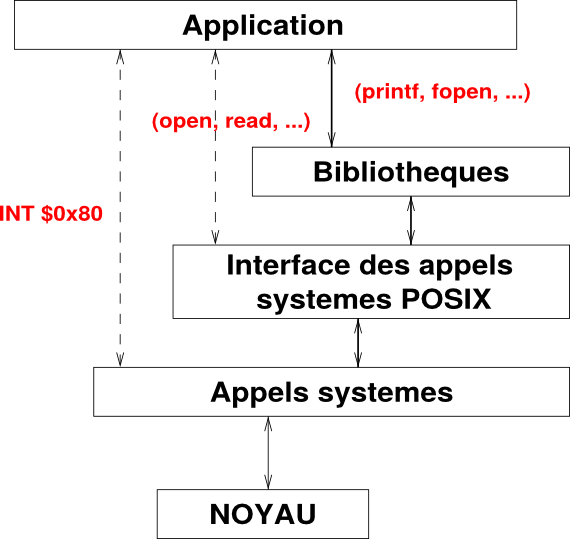
\includegraphics[scale=0.5]{Pictures/Communication_application_noyau_v1.png}
%%  \caption{Communications possibles entre le noyau et une application}
%%  \label{AS_Communication}
%% \end{figure}
\begin{figure}[H]
  \centering
  %\includegraphics[scale=0.40]{Pictures/png/Organisation_generale_code_Simterpose_v22.png}
  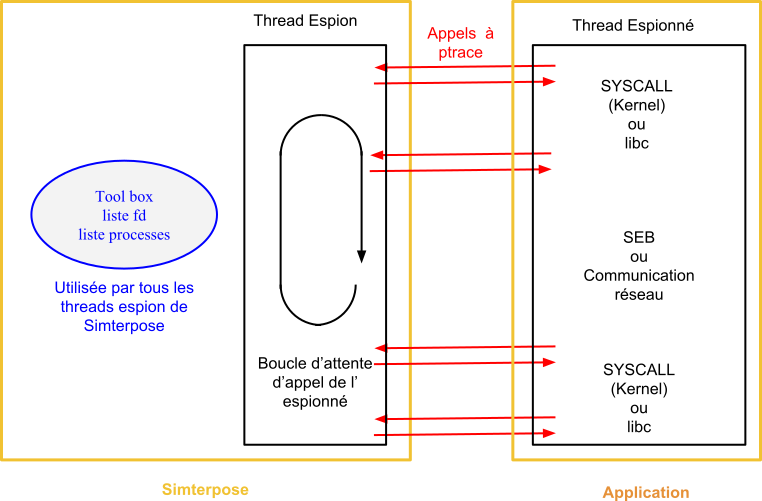
\includegraphics[scale=0.50]{Pictures/png/Organisation_generale_code_Simterpose_v2.png}
      %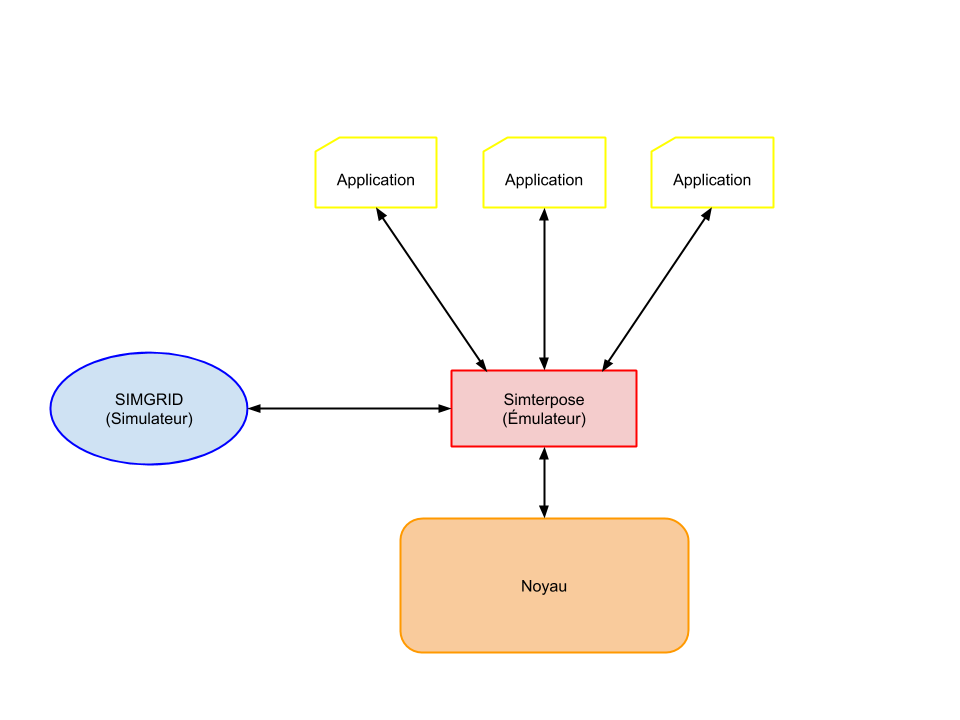
\includegraphics[scale=0.23]{Pictures/png/Simterpose_organisation.png}
  \caption{{\color{red} \textbf{TODO}}}
  \label{Organisation_Simterpose}
\end{figure}

{\color{red} \textbf{TODO}}

\subsection{Les communications réseaux}
 %-> syscall -> ptrace (full mediation, address translation)

Lorsque ptrace est appelé en entrée ou sortie d'appel système, les modifications
à apporter ne sont pas forcément les mêmes selon qu'il s'agit d'une action
nécessitant l'utilisation du réseau ou non. Dans le cas d'un simple calcul ce
qu'il faut maintenir pour l'application, c'est une vision du temps correspondant
à celle qui s'écoulerait si elle était vraiment sur la machine simulée. Ainsi en
entrée d'appel système on n'a pas besoin de modifier quoique ce soit, par contre
au retour il faut modifier le temps d'exécution du calcul en le remplaçant par
celui calculé par le simulateur.

Dans le cas d'une communication réseau, le but de Simterpose étant de réussir à
simuler un réseau réel sur un réseau local, il faut gérer la transition entre
réseau local et réseau simulé. En effet l'application possède une adresse IP et
des numéros de ports virtuels qui ne correspondent pas forcément à ceux
attribués dans le réseau local. De plus on ne peut pas se baser uniquement sur
le numéro de \textit{file descriptor} associé à une socket pour identifier deux
entités qui communiquent entre elles. En effet ce \textit{file descriptor} est
unique pour chaque socket d'un processus, mais plusieurs processus peuvent avoir
un même numéro de \textit{file descriptor} pour des sockets de communications
différentes puisque chacune à son propre espace mémoire. Pour pallier à ce
problème on va utiliser en plus du numéro de socket, les adresses IP et les
ports locaux et distants des deux entités qui souhaitent communiquer comme moyen
d'identification. Pour gérer toutes ces modifications deux solutions ont été
proposées lors d'un précédent stage
\citet{GUILLAUME:Interceptionsyscall}: la \textit{médiation par
  traduction d'adresse} et la \textit{full médiation}.

{\color{red}schéma}
\paragraph{Traduction d'adresse}
 Avec ce type de médiation on considère que le noyau gère des
 communications. Ainsi en entrée et sortie d'appel système Simterpose va juste
 s'occuper de la transition entre le réseau virtuel simulé par SIMGRID et le
 réseau local, en utilisant les informations de communications contenues dans la
 socket. Pour cela, Simterpose gère un tableau de correspondances, dans lequel
 pour chaque couple adresse IP et des ports virtuels, on a un couple adresse IP
 et ports réels sur le réseau associé.  De fait, en entrée d'un appel système de
 type réseau (bind, connect, accept ...), Simterpose doit remplacer l'adresse et
 les ports virtuels de l'application par l'adresse et les ports réels sur le
 réseau local, afin que la source de l'appel système corresponde à une machine
 existante sur le réseau local. Au retour de l'appel système il faudra
 remodifier les paramètres en remettant l'adresse et les ports virtuels pour que
 l'application pense toujours être \textit{dans un environnement distribué.}  La
 limite de cette approche est liée au nombre de ports disponibles sur l'hôte.

\paragraph{Full médiation} 
Dans ce cas, le noyau ne va plus gérer des communications car nous allons
empêcher l'application de communiquer via des sockets et même d'établir des
connexions avec une autre application.  Puisqu'il n'y a aucune communication, on
n'a pas besoin de gérer de tableau de correspondance d'adresse et de ports et
les applications peuvent conserver les adresses et les ports simulées qu'elles
considèrent comme réels. Quand l'application voudra faire un appel système de
type communication ou connexion vers une autre application, le processus espion
de Simterpose qui sera notifié via ptrace neutralisera l'appel
système. \textit{Ensuite, ce processus en utilisant ptrace récupérera, en lisant
  dans la mémoire du processus espionné, les informations à envoyer ou récupérer
  et ira directement les lire ou les écrire dans la mémoire du destinataire.}
Même si la \textit{full médiation} permet d'éviter les communications réseaux et
de conserver des tables de correspondances, elle s'avère moins efficace
  dans le cas d'applications qui communiquent énormément et utilisent de grosses
  données. En effet, les appels à la mémoire sont bien plus coûteux que les
communications réseau.

\subsection{Les thread}
 %% syscall clone + libcalls

\subsection{Le temps}
 %% -> syscall (- system wide), VDSO-linker (cross process ou VDSO)

\subsection{DNS}
%% libcalls (ne rien rater), config fake (system wide), intercept 53 ( plus dur que nécessaire, port dns autre ou pas)
